\section{Обзор Linux}
Linux — общее название UNIX-подобных операционных систем на основе одноимённого ядра и собранных для него библиотек и системных программ, разработанных в рамках проекта GNU.
Система UNIX приобрела популярность в связи с ее успешным использованием на мини-ЭВМ. Этот успех послужил толчком к тому, чтобы создать подобную систему и для персональных компьютеров. Как правило, различные версии ОС, относящихся к этому семейству, имеют свои названия, но в основных чертах повторяют особенности UNIX.

GNU/Linux работает на PC-совместимых системах семейства Intel x86, а также на IA-64, AMD64, PowerPC, ARM и многих других.

UNIX - операционная система, которая позволяет осуществить выполнение работ в многопользовательском и многозадачном режиме. Поначалу она предназначалась для больших ЭВМ, чтобы заменить MULTICS. UNIX является очень мощным средством в руках программиста, но требует очень большого объёма ОЗУ и пространства диска. Несмотря на попытки стандартизировать эту операционную систему, существует большое количество различных его версий, главным образом потому, что она была распространена в виде программы на языке Си, которую пользователи стали модифицировать для своих собственных нужд.

\begin{figure}
	\centering
	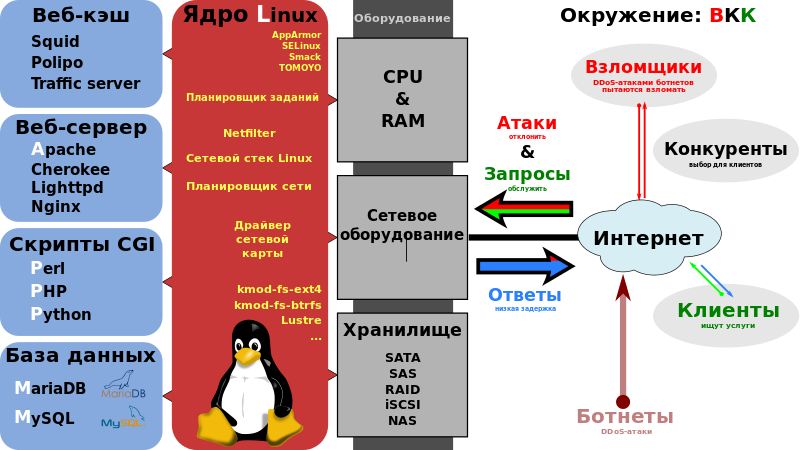
\includegraphics[width=\textwidth]{figures/LAMP_software_bundle}
	\caption{Структура Linux-системы}
	\label{fig:fig01}
\end{figure}

Очень многие считают, что Linux - это только ядро. Но одно только ядро бесполезно для пользователя. Хотя ядро, несомненно, основа ОС Linux, пользователю все время приходится работать с прикладными программами. Эти программы не менее важны, чем ядро. Поэтому Linux - это совокупность ядра и основных прикладных программ, которые обычно бывают установлены на каждом компьютере с этой операционной системой. Объединение ядра и прикладных программ в единое целое проявляется и в названии системы: GNU/Linux. GNU - это проект по созданию комплекса программ, подобного тому, что обычно сопровождает Unix-подобную систему.

Linux изначально был написан Линусом Торвальдсом, а затем улучшался бесчисленным количеством народа во всем мире. Он является клоном операционной системы Unix, одной из первых мощных операционных систем, разрабатываемых для компьютеров, но не бесплатной. Но ни Unix System Laboratories (создатели Unix), ни Университет Беркли, разработчики Berkeley Software Distribution (BSD), не участвовали в его создании. Один из наиболее интересных фактов из истории Linux'а - это то, что в его создании принимали участие одновременно люди со всех концов света – от Австралии до Финляндии – и продолжают это делать до сих пор.

Дистрибутив – это сама ОС + набор пакетов программ для Linux. Стоит также упомянуть, что все это поставляется с исходными текстами, и любую программу, написанную под Linux, можно переделать под себя. Это же позволяет перенести любую программу на любую платформу – Intel PC, Macintosh. Кстати, все вышеописанное получилось благодаря Free Software Foundation, фонду бесплатных программ, который является частью проекта GNU. И именно для этих целей была создана General Public License (GPL), исходя из которой, Linux – бесплатен, как и весь софт под него, причем коммерческое использование программного обеспечения для Linux или его частей запрещено.

Кроме всего ранее упомянутого, Linux – очень мощная и стабильная ОС. Использование его в Сети оправдывает себя, да и взломать его не так уж и легко.

На сегодняшний день, развитие Linux идет по двум ветвям. Первая, с четными номерами версий(2.0, 2.2, 2.4), считается более стабильной, надежной версией Linux. Вторая, чьи версии нумеруются нечетными номерами(2.1, 2.3), является более дерзкой и быстрее развивающейся и, следовательно (к сожалению), более богатой ошибками.

В Linux нет разделения на диски С, D, и процесс общения с устройствами очень удобен. Все устройства имеют собственный системный файл, все диски подключаются к одной файловой системе и выглядит это все как бы монолитно, едино. Четкая структура каталогов позволяет находить любую информацию мгновенно. Для файлов библиотек – свой каталог, для запускаемых файлов – свой, для файлов с настройками – свой, для файлов устройств – свой, и так далее.

Модульность ядра позволяет подключать любые сервисы ОС без перезагрузки компьютера. Кроме того, вы можете переделать само ядро ОС, благо исходные тексты ядра также имеются в любом дистрибутиве.

В ОС Linux очень умело, если так можно выразиться, используется идея многозадачности, т.е. любые процессы в системе выполняются одновременно (сравните с Windows: копирование файлов на дискету и попытка слушать в этот момент музыку не всегда совместимы).

Linux чуть более сложен, чем Windows, и не всем так просто перейти на него после использования окон. На первый взгляд, может даже показаться, что он очень неудобен и труднонастраиваем.

Linux можно настроить под себя, настроить так, что от пользования этой ОС вы будете испытывать огромное удовлетворение. Огромное количество настроек позволяет изменить внешний (да и внутренний) вид ОС. В Linux есть выбор в использовании графической оболочки, есть несколько офисных пакетов, программы-серверы, файерволы.

В 1998 Linux была самой быстро развивающейся операционной системой для серверов, распространение которой увеличилось в том же году на 212 \%.

Сегодня пользователей Linux насчитывается более 20,000,000. Под Linux существует множество приложений, предназначенных как для домашнего использования, так и для полностью функциональных рабочих станций UNIX и серверов Internet.

Если при использовании коммерческой операционной системы пользователь вынужден ждать выхода следующей версии для того, чтобы получить систему без недостатков предыдущей версии, то модульность Линукса позволяет скачать новое ядро, которое выходит не реже раза в два месяца, а то и чаще (стабильная версия). В Линукс-системах пользователи работают через интерфейс командной строки (CLI), графический интерфейс пользователя (GUI), или, в случае встраиваемых систем, через элементы управления соответствующих аппаратных средств.

Настольные системы, как правило, имеют графический пользовательский интерфейс, в котором командная строка доступна через окно эмулятора терминала или в отдельной виртуальной консоли. Большинство низкоуровневых компонентов Линукс, включая пользовательские компоненты GNU, используют исключительно командную строку.

Командная строка особенно хорошо подходит для автоматизации повторяющихся или отложенных задач, а также предоставляет очень простой механизм межпроцессного взаимодействия. Программа графического эмулятора терминала часто используется для доступа к командной строке с рабочего стола Линукс.

Линукс-системы обычно реализуют интерфейс командной строки при помощи оболочки операционной системы, которая также является традиционным способом взаимодействия с системой Unix. Дистрибутивы, специально разработанные для серверов, могут использовать командную строку в качестве единственного интерфейса.

На настольных системах наибольшей популярностью пользуются пользовательские интерфейсы, основанные на таких средах рабочего стола как KDE Plasma Desktop, GNOME и Xfce, хотя также существует целый ряд других пользовательских интерфейсов. Самые популярные пользовательские интерфейсы основаны на X Window System (часто просто «X» или «иксы»). «X» предоставляет прозрачность сети и позволяет графическим приложениям, работающим на одном компьютере, отображаться на другом компьютере, на котором пользователь может взаимодействовать с ними.

Другие графические интерфейсы, такие как FVWM, Enlightenment и Window Maker, могут быть классифицированы как простые менеджеры окон X Window System, которые предоставляют окружение рабочего стола с минимальной функциональностью.

Оконный менеджер предоставляет средства для управления размещением и внешним видом отдельных окон приложений, а также взаимодействует с X Window System. Окружение рабочего стола включает в себя оконные менеджеры, как часть стандартной установки: (Metacity для GNOME, KWin для KDE, Xfwm для Xfce с 2010 года), хотя пользователь при желании может выбрать другой менеджер окон.

Linux работает на множестве процессоров различных архитектур, таких как x86, x86-64, PowerPC, ARM, Alpha AXP, SPARC, Motorola 680x0, SuperH, IBM System/390, MIPS, PA-RISC, AXIS CRIS, Renesas M32R, Atmel AVR32, Renesas H8/300, NEC V850, Tensilica Xtensa и многих других.

В отличие от коммерческих систем, таких как Windows или Mac OS X, Linux не имеет географического центра разработки. Нет и организации, которая владела бы этой системой; нет даже единого координационного центра. Программы для Linux — результат работы тысяч проектов. Некоторые из этих проектов централизованы, некоторые сосредоточены в фирмах. Многие проекты объединяют хакеров со всего света, которые знакомы только по переписке. Создать свой проект или присоединиться к уже существующему может любой и, в случае успеха, результаты работы станут известны миллионам пользователей. Пользователи принимают участие в тестировании свободных программ, общаются с разработчиками напрямую, что позволяет быстро находить и исправлять ошибки и реализовывать новые возможности.